\documentclass[]{final_report}
\usepackage{graphicx}
\usepackage{hyperref}
\usepackage[final]{pdfpages}
\usepackage{booktabs}
\usepackage{multirow}
\usepackage{framed}
\usepackage{caption}
\usepackage{tikz}
\usepackage{xcolor}
\usetikzlibrary{timeline}
\usepackage{dirtree}

%%%%%%%%%%%%%%%%%%%%%%
%%% Input project details
\def\studentname{James King}
\def\reportyear{2018}
\def\projecttitle{Cooperative Strategies in Multi-Agent Systems}
\def\supervisorname{Kostas Stathis}
\def\degree{BSc (Hons) in Computer Science}
\def\fullOrHalfUnit{Full Unit} % indicate if you are doing the project as a Full Unit or Half Unit
\def\finalOrInterim{Final Report} % indicate if this document is your Final Report or Interim Report

\begin{document}

Tips:\begin{itemize}
	\item Communicate with Kostas
	\item Use figures!
	\item Ensure structure is flowing
	\item Use sources for everything
	\item Modularise in order to convert to paper
\end{itemize}
To Do:
\begin{itemize}
	\item Modularise in order to convert to paper
	\item Describe appendix
	\item Act on Interim Review Feedback
	\item Act on planning and timescale comments from interim report
	\item Act on contents of summary of completed work from interim report
	\item Change the Rationale to fit Final report
	\item Write a literature review or combine with Rationale and add to it?
	\item Write Contents and Knowledge
	\item Write critical analysis and discussion
	\item Write professional issues (get background reading and citations)
\end{itemize}
	
\maketitle

%%%%%%%%%%%%%%%%%%%%%%
%%% Declaration

\chapter*{Declaration}

This report has been prepared on the basis of my own work. Where other published and unpublished source materials have been used, these have been acknowledged.

\vskip3em

Word Count: 1,587 \textit{2,000} intro + n \textit{3,000} lit review + n \textit{4,000} framework + n \textit{4,000} experiment evaluation + n \textit{1,000} conclusions + n \textit{1,000} professional issues

\vskip3em

Student Name: \studentname

\vskip3em

Date of Submission: \today

\vskip3em

Signature: \\

\includegraphics[scale=0.05]{Signature.png}

\newpage

%%%%%%%%%%%%%%%%%%%%%%
%%% Table of Contents
\tableofcontents\pdfbookmark[0]{Table of Contents}{toc}\newpage

%%%%%%%%%%%%%%%%%%%%%%
%%% Your Abstract here

\begin{abstract}
\end{abstract}
\newpage

\chapter{Introduction}

\section{Motivation}
Artificial intelligence (AI) has been an idea present in the consciousness of humanity for millennia. From Hephaestus' might Talos to Edgar Allan Poe's commentary on 'Maelzel's Chess-Player' the idea has inspired both awe and confusion. As we move away from the mythical and the false, AI embeds itself deeper into our lives and societies.\\
Intelligent Agents (IAs) and Multi-Agent Systems (MASs) are a key field in close relation to the field of AI. IAs have a range of definitions, but the widest definition was given by Russell and Norvig~\cite{russell2016artificial} as anything that perceives and acts upon its environment. Our world is one of the toughest environments in which we could place an intelligent agent.\\
Advances in software and hardware are taking us closer to perceiving in the real world in the field of computer vision and acting in it in the field of robotics. So we can perceive and act, but there is a big step to acting in a rational manner, defined by Russell and Norvig~\cite{russell2016artificial} as doing the right thing. Rationality is a huge philosophical dilemma, and one that I shall not go into detail about.\\
This step towards rationality is a large part of the study of IAs. However, this does not only include agents set in our world, but also those such as softbots interacting across the internet and various other environments. From the data formulated through perception how can an agent represent the world around it and understand what these perceptions can tell them about their world and from this how can the agent act rationally.\\
One main aim of the study of agent systems is to produce rationally acting agents. In real life rationally acting agents would also need to be socially acting agents in order to reach their goals. In fact, social ability is one of the key properties of IAs laid out by Wooldridge and Jennings~\cite{wooldridge_jennings_1995} and is one of the aspects that is tested in the imitation game~\cite{machinery1950computing}.\\
This is another key area of study for the field of IAs and MASs. Many have marvelled at the development of robotic drones being able to dance through the sky together in beautiful displays. These displays are stunning of course, and if using an agent architecture represent a step towards cooperation between IAs. However, these small societies of drones are programmed to work together most likely by the same people.\\
If artificially intelligent agents are to reach their full potential and integrate into our society, they require the ability to cooperate with agents who can be thought of as `unknown entities' in terms of their intentions. Both the world of the drones and our world can be thought of as MASs. Intelligent agents in our world need to act in the same environment as us and the many different species that also reside on planet earth.\\
As this is one of the final goals of IAs and MASs it appears a natural strategy to use studies of cooperation in the natural world as guidance for the study of IAs and MASs. The early days of evolutionary theory were groundbreaking, but Peter Kropotkin~\cite{kropotkin1902mutual} identified a key flaw in accounting for cooperation between animals.\\
There are many problems to solve before the technology is available to ethically and realistically integrate IAs into our society. The problem I aim to grapple with in this project is how to facilitate cooperation between IAs in MASs.

\section{Aims and Objectives}
The high-level aim of my project is \textbf{to study how developers can facilitate cooperation between IAs and protect them from those with malicious intent}. The objectives to achieve this aim are laid out here.\\
The closest example to a multi-agent system that has allowed cooperation to flourish is that of the natural world. I will be using the study of cooperation in the natural world to inspire my search for a mechanism to facilitate cooperation in MASs. Further to this I will use past studies of multi-agent systems and game theory in regards to the evolution of cooperation. One objective of this study is \textit{to learn about what has previously been identified as possible contributors to the evolution of cooperation}.\\
The deeper objective of this review is \textit{to identify an appropriate mechanism for further in-depth study towards its possible contribution in my high-level aim}. Using a broader study of multi-agent systems as a whole to guide me in this objective.\\
After identifying an appropriate mechanism my next objective will be \textit{to develop a theoretical framework surrounding this mechanism}. Within this framework will be concepts to allow me to study the mechanism and other variables that may have an effect on the evolution of cooperation (such as an agent communication language to study social ability). Furthermore, this theoretical framework will include strategies to associate with agents.\\
My next objective will be \textit{to develop an application that allows a user to set up, simulate and analyse MASs that implement the theoretical framework I have laid out}. This application will aim to allow the user to change the variables previously identified as possible contributors to the evolution of cooperation in order to study them.\\
My high-level aim also includes spreading any knowledge I gain from this study. As such, another objective is \textit{to make the system distributable to people who wish to study the theoretical framework I have outlined}.\\
Using this application my las main objective will be \textit{to examine the relevance and success of the mechanism I have identified to the evolution of cooperation}. I will also use the application to measure how the variables set up in the framework and the various strategies implemented in the program affect the evolution of cooperation. The aim of this is to discover if and possibly how these various aspects can be used to facilitate cooperation between IAs.
To summarise:
\begin{itemize}
	\item Main aim: to study how developers can facilitate cooperation between IAs and protect them from those with malicious intent.
	\item Objective 1: to learn about what has previously been identified as possible contributors to the evolution of cooperation.
	\item Objective 2: to identify an appropriate mechanism for further in-depth study towards its possible contribution in my high-level aim.
	\item Objective 3: identify other factors that may contribute to the evolution of cooperation.
	\item Objective 4: to develop a theoretical framework surrounding this mechanism and other factors.
	\item Objective 5: to develop an application that allows a user to set up, simulate and analyse MASs that implement the theoretical framework I have laid out.
	\item Objective 6: to make the system distributable to people who wish to study the theoretical framework I have outlined.
	\item Objective 7: to examine the relevance and success of the mechanism I have identified to the evolution of cooperation.
	\item Objective 8: to examine the effect of other variables involved in my MAS in regards to the evolution of cooperation.
\end{itemize}

\section{Contribution}
The goal of this project and report is to find areas to explore in regards to facilitating cooperation between IAs. This field is large and a lot of ground has already been covered. I am aiming with the mechanism I identify to find a niche which hasn't been explored as in-depth as other areas, either specifically with the mechanism or a combination of the central mechanism and a number of other factors.\\
As such I aim to create a theoretical framework that is unique. This will allow me to examine some less explored factors for the evolution of cooperation, and hopefully find some interesting results as to how they affect cooperation among IAs.\\
Another contribution I am aiming to make is to make the application I develop distributable. This has been done by others such as the Python Axelrod library~\cite{axelrodproject} and the evolution of trust website~\cite{evol_trust}, but I hope to introduce a less Iterated Prisoner's Dilemma focused mechanism.


\section{Structure}
The structure of this report is to follow the objectives laid out above. First I will conduct a literature review to conquer the objectives 1-3. This literature review will help me conduct research into the field and gain an in-depth understanding of what experiments have taken place and what ideas have been put forward. On review of the literature, I will be gaining an understanding also of what has not been explored and/or what could do with a more in-depth exploration. From this, I will be able to identify what mechanism and which factors to use in my theoretical framework.\\
This leads me nicely into my framework section which aims to tackle objectives 4-6. Here I shall use the mechanism and factors I have identified to lay out a framework with which I wish to experiment. This framework will aim to suit the arena of MASs and be examinable in terms of the factors I have identified. The next part of my framework section will be in regards to the implementation of this theoretical framework. This will be in an application that is distributable to people interested in the problem and framework.\\
Once I have designed, implemented and tested this application, I will be using it for objectives 7 and 8. For these objectives, I will conduct a number of experiments to analyse both the mechanism and the factors built into the theoretical framework. To do this I will be controlling variables using the applications set up phase and then reviewing the outcome using the analysis phase. I will then discuss and analyse the results of these experiments.\\
This discussion and analysis will drive my conclusions at the end of the report.


\chapter{Background}
\section{Introduction}
The evolution of cooperation between individuals is a keenly studied topic, as such there is a large set of related literature. Approaches to the problem have come from areas such as biology, social systems, game-theory and of course IAs and MASs. This background section will be a review of past literature in the topic, with a view to exploring the best options for facilitating cooperation in MASs.\\
The literature review will be tackling the first 3 objectives from my introduction. As such, the outcomes of this literature review will be a knowledge of the current explorations of the evolution of cooperation, a decision on which mechanism to use to facilitate cooperation and factors to study that may aid or discourage the evolution of cooepration in a MAS.\\
\\
Include background reading\\
Critical lit review.\\
Comprehensive knowledge.\\
Objectives 1-3.\\
Examples:
\begin{itemize}
	\item Evolcoop Axerlrod, Axelrod.py
	\item Arithmetics of mutual help
	\item Pheklps, game theoretic analysis
	\item 5 rules coop
	\item spatial and graphs
	\item multilevel nowak
	\item Genetic drift as an issue
	\item gossip alternative
	\item rational cooperation in finite iterated prisoners
	\item prisoners and their dilemma
	\item evol dir indir
	\item evol of coop through indir rec
	\item kin hamilton
	\item image vs standing
	\item notions of reputation in mas
\end{itemize}

\section{Cooperative Phenomena}
Russell and Norvig~\cite{russell2016artificial} describe an agent as being able to interact with their environment, but more interesting MASs also allow interaction between agents. Cooperative actions occur in interactions between agents, where the action of one benefits another at a loss to the actor. A defection is the opposite of cooperation, in the way that the action does not benefit the recipient of the action, but it is not a loss to the actor. This cooperative phenomena is also present in biology.\\
Early evolutionary theory struggled to explain why cooperation is so prevalent in nature~\cite{spencer1864principles}. Axelrod and Hamilton~\cite{evolution_of_cooperation} note two key areas of study that attempt to explain cooperation: kinship theory and reciprocal altruism. As they are useful for explaining cooperation in nature, there is a good possibility they can be applied to MASs in order to facilitate the evolution of cooperation between agents.

\section{Kinship Theory}
\label{sec:kin}
Axelrod and Hamilton~\cite{evolution_of_cooperation} described the way in which cooperation in nature (with the exception of homo sapiens) is almost always between related individuals. An earlier paper by Hamilton~\cite{kinhamilton} argues that individuals don't only work toward improving their own fitness, but what Hamilton defines as `inclusive fitness'. Inclusive fitness is the sum of the players fitness and the fitness of each of their relations multiplied by a coefficient. The coefficient used by Hamilton is Wright's coefficient of relatedness. It could be possible to create a similar coefficient of relatedness for use in a MAS.\\
Richard Dawkins~\cite{selfish_gene} advocated for the idea of the selfish gene. From a biological perspective this is the idea that actors are hardwired to propagate their genes. This is due to genes being the true replicators evolutionarily rather than the actors themselves. This idea from a biological sense is well thought of, however, it does not seem natural to translate an agents strategy to the idea of genes.\\
Though it could be possible to create a coefficient and an idea of relatedness similar to Hamilton's model~\cite{kinhamilton} for MAS, this does not seem a natural translation. Another limitation to the use of kinship theory for MASs is that we want our systems to be inclusive of individuals that can contribute to our society of agents. Not cooperating with agents that would contribute to a society, but are not kin with the members of that society is uninclusive and limits the abilities of that society.\\
Furthermore Axelrod and Hamilton~\cite{evolution_of_cooperation} highlighted that humanity is the exceptional society which does not limit itself to cooperating mostly only with kin. I would surmise that this is due to the higher level of intellect of homo sapiens in comparison to other species. Many have suggested that the capabilities of AI could match if not surpass the intelligence of humans, so I would suggest that societies of IAs will also not be limited to the use of kinship theory to facilitate cooperation.\\
Due to these reasons I shall not be using kinship theory for my theoretical framework. I will be aiming to use a  mechanism that is inclusive of any agent that aims to be a valuable member of the society and also a mechanism which fits naturally into the agents paradigm. 


\section{Reciprocal Altruism}
Reciprocal altruism is an idea most famously put forward by Robert L. Trivers~\cite{trivers1971evolution}. Trivers defines altruism as behaviour that benefits another organism, not closely related, while being apparently detrimental to the organism performing the behaviour. From this definition and Trivers' description of human reciprocal altruism we can draw the meaning of reciprocal altruism to be altruism based on the idea that the altruistic act will be returned.\\
This is a move away from limiting individuals to cooperating with only their kin towards any individual that they believe will reciprocate their cooperation. Axelrod and Hamilton~\cite{evolution_of_cooperation} noted this as an advantage in explaining cooperation between unrelated individuals, such as is common between humans. I would argue that this makes it more applicable to higher intelligence societies such as those possible from IAs.\\
In comparison to kinship theory this seems the more natural match to the agents paradigm - not requiring measures for relatedness between agents or conversion between an agents strategy and the concept of a gene. Reciprocal altruism is the more likely to apply to my problem.

\section{Axelrod, Hamilton and The Iterated Prisoner's\\ Dilemma}
\label{sec:ipd}
Axelrod and Hamilton~\cite{evolution_of_cooperation} also chose reciprocal altruism for further study over kinship theory. They recognised kinship theory limited individuals to only cooperating with kin and at the time more investigation had been into kinship theory. Of course the same cannot be said now, a lot of investigation has gone into reciprocal altruism a lot of this due to their paper.\\
Game-theoretic modelling was used by Axelrod and Hamilton~\cite{evolution_of_cooperation} making use of The Iterated Prisoner's Dilemma. This dilemma makes use of direct reciprocity. The Dilemma can be though of by imagining that a crime has been committed by 2 individuals who are now being interviewed by the police. Each individual can either choose to inform on the other, or stay loyal and say nothing.\\
Staying loyal is known as cooperating, informing is defecting. If an individual informs on the other they will receive a lower sentence, as long as the other has stayed loyal. However, if both defect they both receive a bad sentence, but, not as bad as the individual who stays loyal when the other defects.\\
If this dilemma is not repeated a defector can get away with defecting and is never punished for this. However, if the game is repeated in multiple the mechanism of direct reciprocity comes into player. This is the idea that if I cooperate with you, you will cooperate with me in later rounds~\cite{five_rules_coop}. Across multiple rounds when an individual doesn't know which round will be last it may be more beneficial for them to cooperate. This encourages selfish players to cooperate.\\
The focus of Axelrod and Hamilton's paper~\cite{evolution_of_cooperation} is to review the strategies of The Dilemma submitted to them by academics and teams working on the strategies throughout the world. They asked 3 questions of each strategy. Is the strategy robust? Is it stable? Is it initially viable?\\
Robustness is the ability to thrive in an environment with a variety of strategies. Stability is the ability to - once fully established - resist invasion by mutant strategies. Initially viability is whether or not a strategy can establish itself is a noncooperative environment.\\
They found two strategies with these 3 abilities: tit-for-tat and all defect. Later on Nowak and Sigmund~\cite{nowak-1993a} found that Pavlov (win-stay, lose-shift) also has these abilities. The interesting part of Pavlov and tit-for-tat is that they are nice strategies (start by cooperating) and that they actively aid in the evolution of cooperation.\\
Another key part of The Iterated Prisoner's Dilemma is the way in which it has been formulated by Axelrod and Hamilton~\cite{evolution_of_cooperation}. In each round players simultaneously either choose to cooperate, the players earn points based on the outcome of the game as given in the payoff matrix in figure~\ref{tab:payoffmatrix}. Nowak~\cite{five_rules_coop} found that for the evolution of cooperation to occur the cost-to-benefit ratio ratio of the altruistic act must be less than the probability of another encounter for cooperation to evolve: $w>c/b$.\\
\begin{framed}
	\begin{center}
		\begin{tabular}{c|c|c}
		\multirow{2}{*}{Player A} & \multicolumn{2}{c}{Player B}\\		
		& Cooperation & Defection\\
		\hline
		\multirow{2}{*}{Cooperation} & A=3 & A=0\\
		& B=3 & B=5\\
		\hline
		\multirow{2}{*}{Defection} & A=5 & A=1\\
		& B=0 & A=1\\
		\end{tabular}
		\captionof{table}{The payoff matrix in a typical iterated prisoner's dilemma game (such as Axelrod and Hamilton's). A=x, B=y where x denotes the payoff for A and y the payoff for B.}
		\label{tab:payoffmatrix}
	\end{center}	
\end{framed}
If the probability of another encounter between two individuals is low, it is very likely that cooperation will not evolve as there is no sufficient reward for it. With the advent of huge networks spanning across the world and the drastic increase in devices across these networks, it is highly likely MASs will operate with IAs that are unlikely to meet again.\\
This is a definite limitation to the use of direct reciprocity in MASs, and as such I do not see it as a good contender to encourage cooperation in MASs on it's own. One property of a mechanism to encourage cooperation is that it must work when both re-meeting is unlikely and when it is likely. So this does not mean to say that direct reciprocity is completely inadequate for the problem, but that it is insufficient when not combined with some other mechanism for when re-meeting chances are low.\\
Another reason for not further studying this mechanism is that a lot of the interest in reciprocal altruism has focused on The Iterated Prisoner's Dilemma. This includes a number of libraries that are available such as the Axelrod Python library~\cite{axelrodproject}. I argue that to gain a better understanding of how we can work to facilitate cooperation between IAs we must look at a wider berth of options.

\section{Network Reciprocity}
Nowak~\cite{five_rules_coop} identified and compared 5 key mechanisms that can aid in the evolution of cooperation, 2 of which I have already discussed (direct reciprocity in section~\ref{sec:ipd} and kin selection~\ref{sec:kin}). The other 3 are network reciprocity (which I shall be examining here), group selection and indirect reciprocity (both of which have their own sections).\\
Network models a graph of connected players. The players are the nodes in the graph and the arcs between them represent connections between players. This ties closely to the networks that IAs may work across. Players with arcs between them interact with each other in rounds of The Prisoner's Dilemma. Nowak and May's~\cite{spatial} ealier work that inspired Nowak's later paper~\cite{five_rules_coop} did not give individual's any memory of past interaction.\\
The lack of memory limited Nowak and May to pure cooperators and pure defectors. In Nowak's book `Evolutionary Dynamics'~\cite{nowak2006evolutionary} his exploration of evolutionary graph theory and spatial games (chapters 8 and 9) showed that the shapes of the lattice linking the players and different concentrations of cooperators and defectors on those shapes has a great effect on the evolution of cooperation.\\
Nowak's~\cite{five_rules_coop, nowak2006evolutionary} and Nowak and May's~\cite{spatial} work on the games on graphs is limited in terms of it's strategies and in terms of the fixed shape of it's graphs. But the work proves a key point: the structure of who interacts with whom can play a key role in supporting cooperation in large populations.\\
I can imagine the use of their work to employ a network not as a representation of a physical network structure such as the internet as I first thought, but as a representation of the choices IAs make on who they wish to interact with. This would be a constantly changing and adapting network of IAs that do not concern themself with the strategy they employ towards who they are forced to interact with, but, their key strategy is to build a network that suits their purposes. How these changing graph connections would effect cooperation is unbeknownst to me, whether Nowak's rules would still apply would be interesting to find out.\\
Nowak~\cite{nowak2006evolutionary} found some shapes supported cooperators in groups, cooperators could make use of these shapes by deliberately forming them to protect each other. While another set of shapes were found as `amplifiers' for evolution, maybe defectors could make use of these sorts of shapes to invade groups of cooperators.\\
I can see IAs having strategies as to how to build these shapes. However, I see one issue that cooperative agents may find it hard to reach out to other cooperators not part of their current shape. This could possibly prevent the spread of cooperation, and limit it to these groups. This is however worth investigating, and possibly may involve some kind of bridging mechanism.

\section{Group Selection}
Group selection technique, limitations, our work

\section{Indirect Reciprocity}
~\cite{alexander1987biology}.\\
Conclude as to why I'm choosing indirect reciprocity.

\section{Nowak and Sigmund}
According to Gilbert Roberts~\cite{evoldirindir} the most influential model on indirect reciprocity Nowak and Sigmund's~\cite{evol_indirect_image} so I shall examine this model of indirect reciprocity first. Nowak and Sigmund begin by stipulating that human cooperation is not due to kin selection as much as it is due to the `image' of each person. This `image' is comparable to the idea of reputation. However, this image is translatable to an integer score between -5 and 5 according to Nowak and Sigmund.\\
The theory is dubbed an extension or subgroup of reciprocal altruism by Nowak and Sigmund. In the context of indirect reciprocity reciprocal altruism is the act of cooperating with one player in expectation of receiving a cooperation from others. Nowak and Sigmund highlight that this channels cooperation to valuable members of the society of players.\\
These players are generally to be more `sophisticated' in comparison to those that fit into the direct reciprocity category according to Nowak and Sigmund. Due to this they mark out that anticipation, planning, deception and manipulation are likely to have a big effect on the system. These 4 concepts seem closely related to possible happenings in MASs. Deception and manipulation are two factors that I will be experimenting with.\\
The framework created by Nowak and Sigmund is simplified from Alexander's~\cite{alexander1987biology} idea of human reciprocal altruism. They describe a framework where there is a population of individuals which is a effectively acts as a pool to select pairs in which one player is the donor and can choose whether to cooperate or defect and the other is the recipient of this action. A cooperation costs the donor $c$ to it's fitnss and benefits the recipient's fitness the value of $b$ where $b>c$. Whereas a defection costs nothing and the recipient is not benefitted.\\
These fitness scores are not the only effect of the actions. A cooperation increases the donor's image score by 1 and a defection decreases it by 1. Nowak and Sigmund add a caveat on top of this when using the idea of onlookers. Onlookers limits the players that can view a particular interaction to only some of the population, and as such the image scores are stored in a matrix $ImageScore$ where each individual has an image score for every other individual.\\
The discriminator is the sophisticated strategy of choice for Nowak and Sigmund. This strategy stores a number $k$, and when the individual $u$ using that strategy is a donor to the individual $v$, $u$ cooperates when $ImageScore[u,v]>=k$. This model also includes the defector and cooperator strategies. Nowak and Sigmund also detailed another set of strategies, that based their decisions not only on that of the recipient's image score but also their own. This way the individual will be able to decide whether they need to boost their reputation in the system or not.\\
Nowak and Sigmund hypothesize and give evidence supporting that the length of the generation is important to the evolution of cooperation. They highlight that when $m$ donor-recipient pairs are selected in succession in a population of size $n$ a player is likely to be selected as part of a pair $2m/n$ times. According to their evidence the higher this value of $2m/n$ the more likely cooperation will evolve. The length of the generation is another variable I will be testing as to its significance in my framework.\\
Herbert Spencer coined the phrase ``Survival of the fittest''~\cite{spencer1864principles}. This is a principle used by Nowak and Sigmund in terms of their reproduction mechanism. The higher the fitness of an individual the more likely it is they will reproduce into the next generation in their mechanism. This is a principle which I will be using in my reproduction mechanism. This mechanism also includes a chance for random mutation.\\
Another idea put forward and evidenced by Nowak and Sigmund is that the evolution of cooperation is dependent upon the ability of the donors knowing the image score of the recipient. This chance of knowing an image score correctly is limited by the concept of onlookers, but, in Nowak's 2005 paper on the five rules of cooperation~\cite{five_rules_coop} he talks about using `gossip' as an alternative to direct observation. Gossip and social ability is a concept I will be exploring further.\\
Nowak and Sigmund stress that discriminators are not tit-for-tat players as used in direct reciprocity, as they use the experience of others. This is true however the similarity lies in the way that discriminators punish those with lower image scores because of their bad actions, but are forgiving to those who improve and cooperative to those who cooperate with them.\\
The model laid out by Nowak and Sigmund is succinct and a good simple basis for looking at interactions in multi-agent systems. However, there are limitations to their approach in the context of MASs. The first limitation I will highlight is the way in which reputation is implemented. In the version without onlookers each player has a global image score and even in the version with onlookers there is a matrix encoding all image scores.\\
Image score could be seen as a community view on an individual, but I argue that the idea image scores are attempting to capture (reputation) is actually more personal. Though there might be a rough consensus as to an individuals' general reputation among people in a society, this reputation is often conveyed through social means and is subject to the personal interpretation of each individual.\\
According to Russell and Norvig~\cite{russell2016artificial} IAs use an internal state to encode what might be considered their `beliefs' about their world. It is in this internal state I argue that image scores for those an agent has encountered should be stored, where an agent has full control over their image score of another. This is a closer match to the agent paradigm.\\
Further to this the use of a central matrix would prevent a MAS from being truly distributed in practice. Leimar and Hammerstein~\cite{leimarhammer} criticised Nowak and Sigmund's limited range of strategies. I think this is a fair criticism and as such will be endeavouring to include more strategies in my model including that of both image scoring and standing strategies~\cite{sugden2004economics}.\\
Indirect reciprocity makes a good candidate for use in MASs and this model is both very influential and a good basis for those MASs. As such I will be using a lot of the ideas laid out by Nowak and Sigmund including the use of onlookers, fitness scoring and a reproduction mechanism inspired by Herbert Spencer~\cite{spencer1864principles}, an altered version of their discriminator strategy, the donor-recipient pairs in successive timepoints taken from a population pool and Nowak and Sigmund's payoff system.\\
I will also be looking at employing a number of ideas Nowak and Sigmund discussed but did not fully test including that of using gossip to spread reputation information and how deception and manipulation (including using gossip) can affect a system using indirect reciprocity. My system's key difference will be to leave the interpretation of events down to the strategy an individual is using, and store them in the agents' internal state.

\section{The Standing Strategy and Further Limitations of Nowak And Sigmund}
As discussed by Nowak and Sigmund~\cite{evol_indirect_image} there is another popular strategy in indirect reciprocity known as the standing strategy. This was first described by Sugden~\cite{sugden2004economics} and is described as using a switch by Nowak and Sigmund.\\
Milinski \textit{et. al}~\cite{imagevsstanding} described standing as the idea is that an individual does not only aim for a good fitness but also a good standing. Each individual holds other individuals in either a good or bad standing, and this standing starts out good until events perceived show otherwise. The event that causes the switch from good to bad standing of an individual is defecting against a good individual.\\
The idea is that it is morally incorrect to defect against a good individual, but defecting against a bad individual is acceptable as it punishes those members of society that are not valuable to the society. There is conflict between the use of image scores and the standing strategy. Leimar and Hammerstein~\cite{leimarhammer} argue that Sugden's version of indirect reciprocity and his use of the standing strategy are more robust than Nowak and Sigmund's image scoring.\\
Milinski \textit{et. al}~\cite{imagevsstanding} analysed Leimar and Hammerstein's argument, regarding that they were correct under conditions which allowed for perfect perception of events and unlimited memory capacity. Nowak and Sigmund claimed that indirect reciprocity is open to deception and manipulation, especially when we consider the use of gossip in a system. This opens IAs to imperfect perception of other IAs. So it will be interesting to see which strategy is more effective in a system where other IAs actively attempt to deceive using gossip.

\section{Mixed Reciprocity Models}
Roberts~\cite{evoldirindir} and Phelps~\cite{phelps_game_theoretic_analysis} noted that indirect reciprocity is focused towards interactions with other individuals that the donor has no previous interactions with. But what about when re-meeting is more likely? Surely an individual is affected by both being the recipient of actions and observation of actions. Roberts tackled the issue by introducing an experience score. This experience score works similar to an image score, but is bounded by -1 and 1, it increases when the individual is a recipient of a cooperation, and decreases when receiving a defection.\\
Both Roberts and Phelps measured the use of indirect reciprocity vs the use of direct reciprocity. Roberts concludes that indirect is the more popular decision mode under conditions when re-meeting was less common, and direct was more common when re-meeting was frequent. Whereas, Phelps' experiments garnered different results being that in small groups direct and indirect reciprocity exist in equilibrium.\\
Just like in Nowak and Sigmund~\cite{evol_indirect_image}, Roberts I believe falls short in recognising how personal interpretation of events are. Roberts creates a version of the standing strategy which uses an image score, but the image score changes according to the rules of the standing strategy rather than Nowak and Sigmund's rules.\\
There are many different trust models a player could use by mixing interpretation of events where they are the recipient and when they are not the recipient. For example it could be expected that being on the receiving end of a defection a player is likely to be more hardline, than when they observe a defection against another. Whereas Roberts limits the study to using a simple experience score.\\
My model will leave interpretation of events up to the individual's strategy and as such will be extensible in terms of adding trust models for both events directly affecting them and observed events. This will effectively make the model a form of mixed reciprocity.

\section{Gossip}
Nowak and Sigmund~\cite{evol_indirect_image} realised the issues surrounding all individuals being able to view interactions in their simulation framework. So they introduced the idea of onlookers as noted above. An issue with limiting observation is that knowing an accurate image score of a player is important to the evolution of cooperation in an indirect reciprocity system. Nowak~\cite{five_rules_coop} suggested using gossip to spread information regarding image scores in their simulation framework.\\
Sommerfeld \textit{et al.}~\cite{gossip_alt} conducted an empirical study on gossip between cooperative and uncooperative individuals in an indirect reciprocity setup. The experiment consisted of humans playing a number of indirect reciprocity rounds to build up a cooperation history, and then a smaller number of gossip rounds. These rounds are then repeated to see how the individuals reacted to the gossip.\\
The focus of the experiment was to look at gossip composition, gossip transfer and the resulting behaviour. Sommerfeld \textit{et al.}~\cite{gossip_alt} concluded that gossip is an effective method of spreading reputation information in an indirect reciprocity system, on fulfillment of some conditions. The first of which is truthfulness of the gossip. Gossip must accurately reflect the behaviour of the subject of the gossip.\\
Another condition is the comprehensibility of the gossip. The language used in the gossip must be interpretable by the recipient of the gossip. In an agent system this would require an agent communication language (ACL) and content of the messages that use this language to be understandable by the recipient agent. The final condition is that individuals must act accordingly based on the gossip they receive.\\
These three key conditions of a system would have to be created by building strategies for agents that attempt to uphold them, and a communication language to support accurate and interpretable information. Nowak and Sigmund~\cite{evol_indirect_image} identified that indirect reciprocity systems can be effected by deception and manipulation by possibly malicious players. The addition of gossip creates a meta-game on top of the indirect reciprocity system where players must have a strategy to decide whether to trust gossip and how to spread gossip effectively.

\section{Mui's Computational Models of Trust and Reputation}
Mui~\cite{mui2002computational} presented an indirect reciprocity simulation framework similar to Nowak and Sigmund~\cite{evol_indirect_image} that spread social information through `acquaintance networks' to inform a donor's decision. An individual in this framework builds up a network of players' they meet through interactions called an `acquaintance network'. If this individual is then a donor in a donor-recipient pairing they consult their acquaintance network about the recipient.\\
The information gathered from this network helps a donor decide if they can trust the recipient to reciprocate their cooperation. Mui refers to this gathered information as `collective memory'. Baumeister \textit{et al.}~\cite{baumeister2004gossip} advocated for the idea that gossip is used for 4 functions. These 4 are strengthening bonds between the gossiper and recipient, enabling the spread of information about the subject for both positive and negative reasons, and to help educate individuals about the complex cultural systems they reside in.\\
I would argue that indirect reciprocity systems and MASs are complex cultural systems in which gossip can be applied for these 4 functions. Mui's acquaintance networks support this gossip functionality to a certain extent but are limited by the lack of proactivity of the gossip. Sommerfeld \textit{et al.}~\cite{gossip_alt} highlighted the willingness of their participants to spread gossip and the last function of gossip proposed by Baumeister \textit{et al.}~\cite{baumeister2004gossip} (cultural education) suggest that for gossip to be most effective the gossip should be proactively spread.\\
As a result of this I will be presenting a theoretical framework that promotes active social gossip by using gossip as an action at times when an agent is not acting as a donor. 

\section{Summary}
Decide on indirect vs. network reciprocity.\\
Summarise limitations and the techniques we are using to combat this.\\
List identified mechanism and other factors.

\chapter{Framework}
Excellent understanding and insight. Conceptual framework underpins study. Comprehensive expert account of topic. Well thought through Software Engineering content.

\section{Theoretical}
Relate to background.\\
Simple agent gossip language (SAGL).\\
Actions.\\
Environment. Generations and Communities.\\
Agent design. Strategy + trust model.\\
Onlookers.\\
Objective 4.\\
Look at summary of Lit review + end of each section of lit review


\section{Implementation}
Relate to agents systems.\\
Making it distributable.\\
Objectives 5 and 6\\
AMAAS.\\
Logic framework


\subsection{Agent Mind as a Service}
\subsection{Environment}
\subsection{Web Application and Interface}
\subsection{Conclusion}

\section{Technical Preparation}
Learning flask etc.

\section{Design}

\subsection{Agent Mind as a Service}
\subsection{Environment}
\subsection{Web Application and Interface}

\section{Development}

\subsection{Agent Mind as a Service}
\subsection{Environment}
\subsection{Web Application and Interface}

\section{Testing}

\subsection{Agents Service Testing}
\subsection{Environment Testing}
\subsection{Web Application Testing}

\section{Software Engineering}

\section{Documentation}
Software documentation, user guide.

\chapter{Experiment Evaluation}
\section{Introduction}
What experiments will I be doing, why?\\
Factors that could effect cooperation:
\begin{itemize}
	\item Number of generations
	\item Strategy
	\item Trust Model
	\item Whether a player knows the reputation of another player (generation size, generation length (2m/n~\cite{evol_indirect_image}), onlooker number and social activeness)
	\item Positivity of gossip vs Accuracy of gossip
	\item Deception and manipulation (image vs standing)
	\item Sommerfeld's 3 properties
\end{itemize}
Control variables:
\begin{itemize}
	\item Number of generations
	\item Mutation chance
	\item How many experiment repetitions? ( due to non-determinicity of the game)
\end{itemize}


\section{Experiment 1}
Variable setting, controls etc.\\
Evaluation

\section{Experiment 2}

\section{Experiment n}

\section{Discussion}
Evaluation and discussion on the experiments\\
Successful?\\
Opportunity for extra work?\\
Focus on experiments

\chapter{Critical Analysis and Discussion}
Project achievements\\
Reflection on project process (difficulties, success, failure)\\
Successful?\\
Future enhancements\\
Focus on project\\
Compare to deliverables at beginning.

\chapter{Conclusions}
Mechanism has to work with and without re-meeting.\\
Mechanism has to encourage cooperation between unknown entities.\\
Opportunity for extra work? Further exploration of complex network reciprocity (from Nowak's five rules section).\\


%%%% ADD YOUR BIBLIOGRAPHY HERE
\newpage
\bibliography{../../refs.bib}{}
\bibliographystyle{plain}
\addcontentsline{toc}{chapter}{Bibliography}
\footnote{A lot of my background theory work has been completed in my earlier reports so many of the references appear in those reports (see appendix)}
\label{endpage}

\chapter{Professional Issues}
Replacement of people in jobs?\\
AI issues and risks?\\
Relate to project\\
Moral philosophy of agent societies

\chapter{Appendix}
\label{appendix}
Describe the contents of my appendix.

%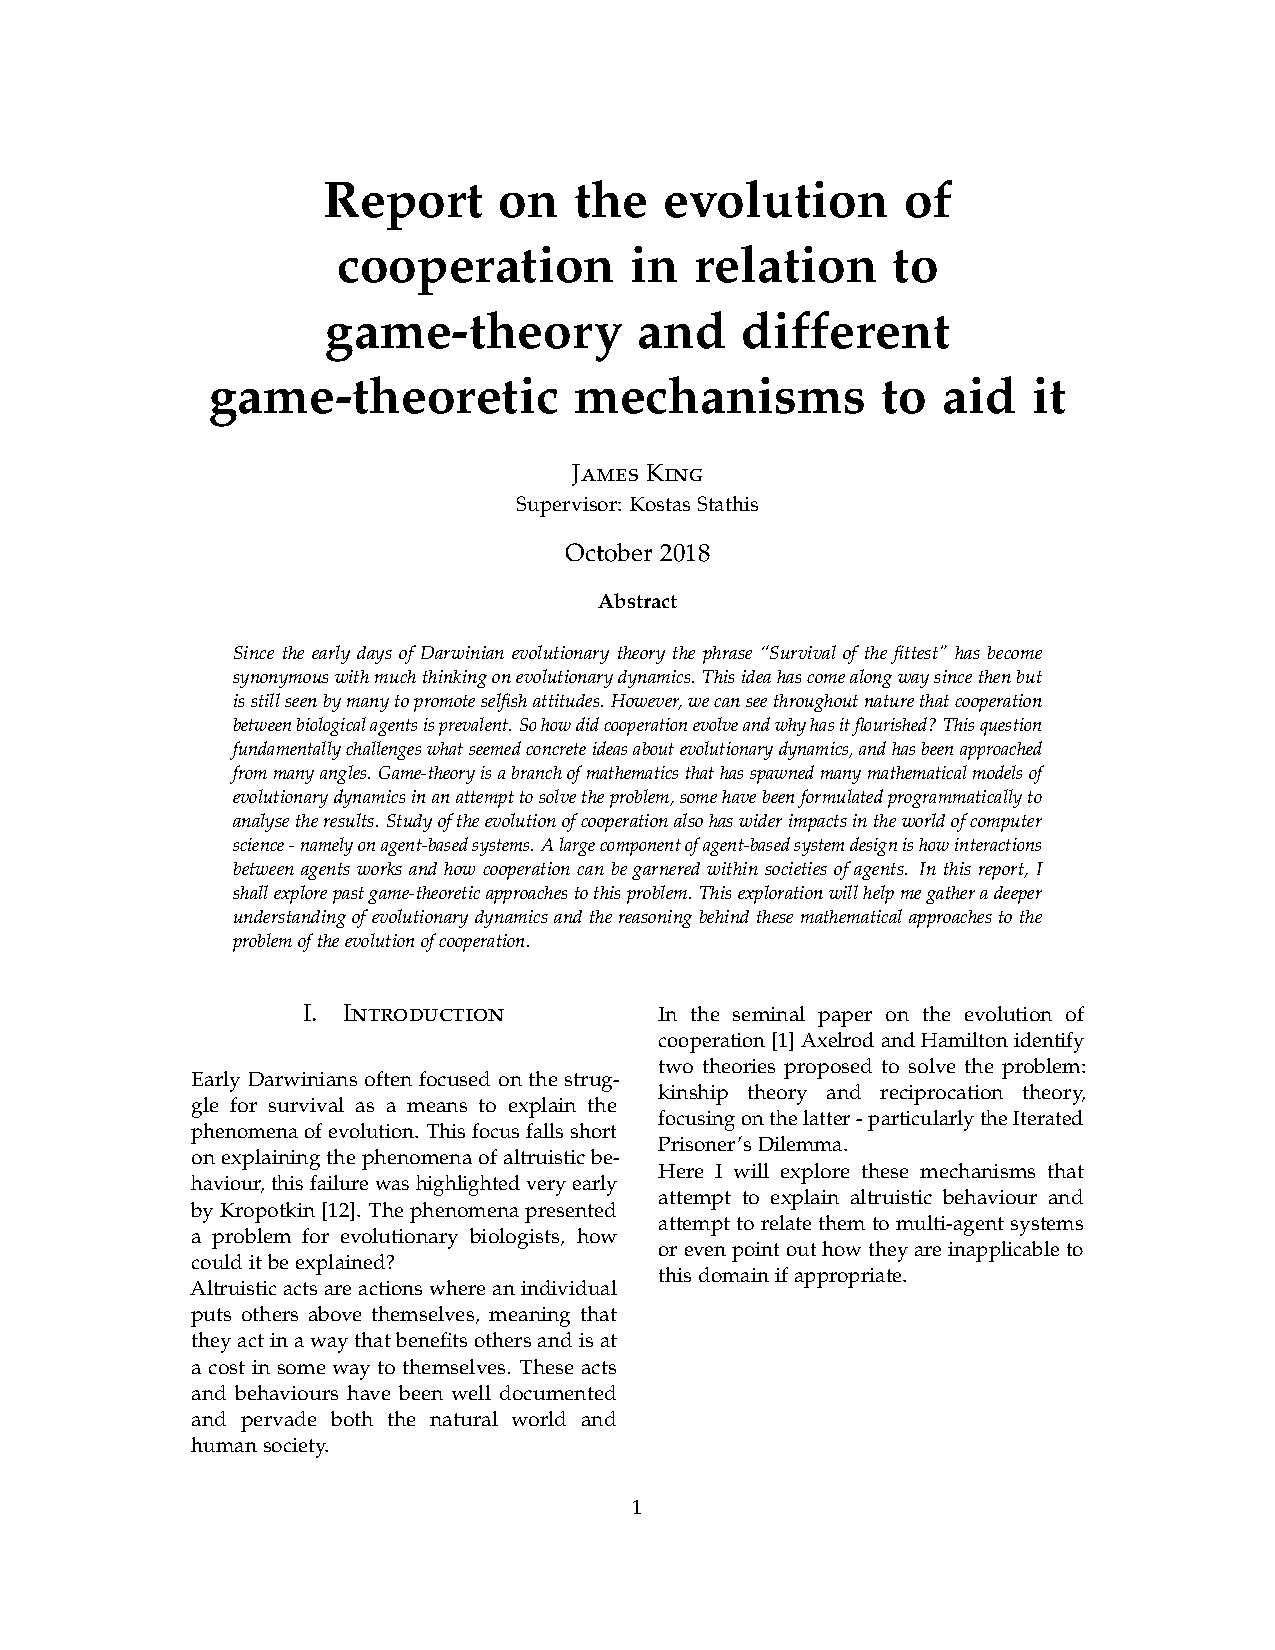
\includepdf[pages=-]{../../EvolCoop/EvolCoopReport.pdf}

%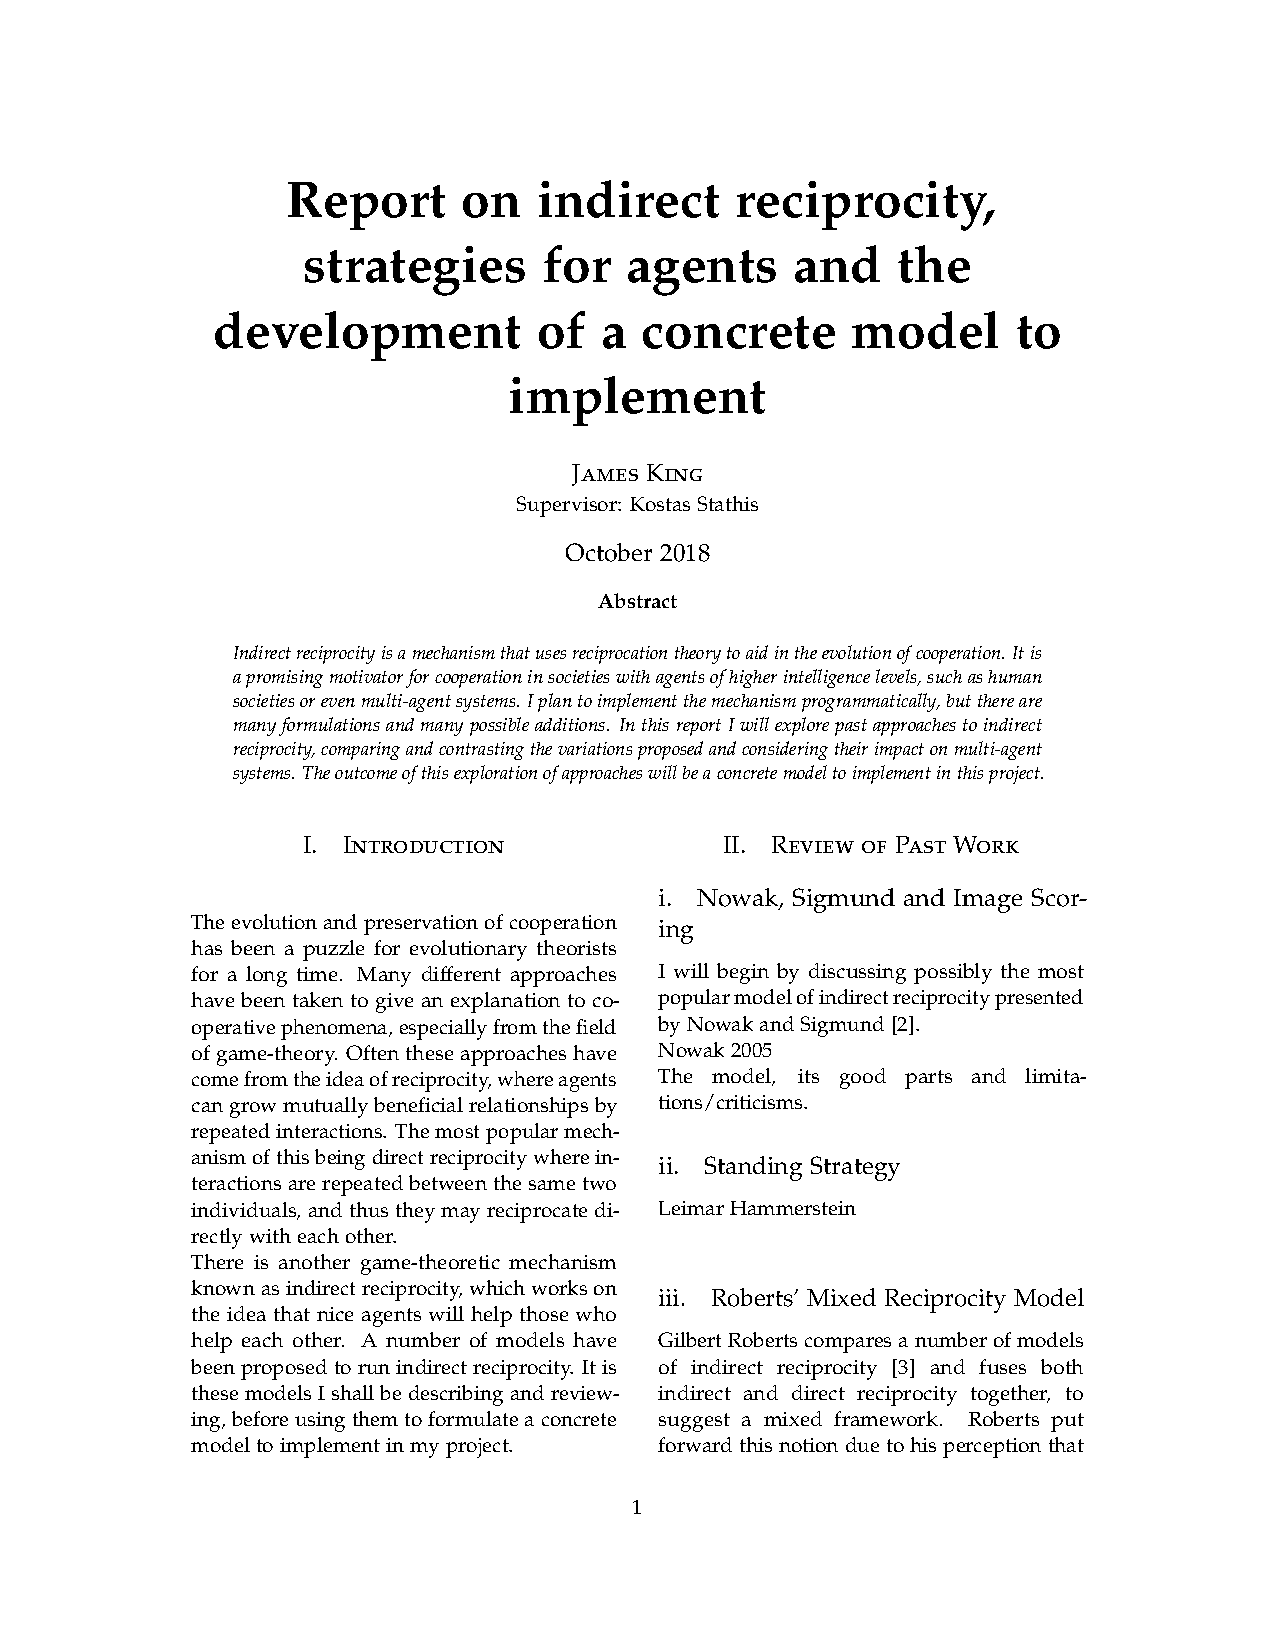
\includepdf[pages=-]{../../IndirRec/IndirRec.pdf}

%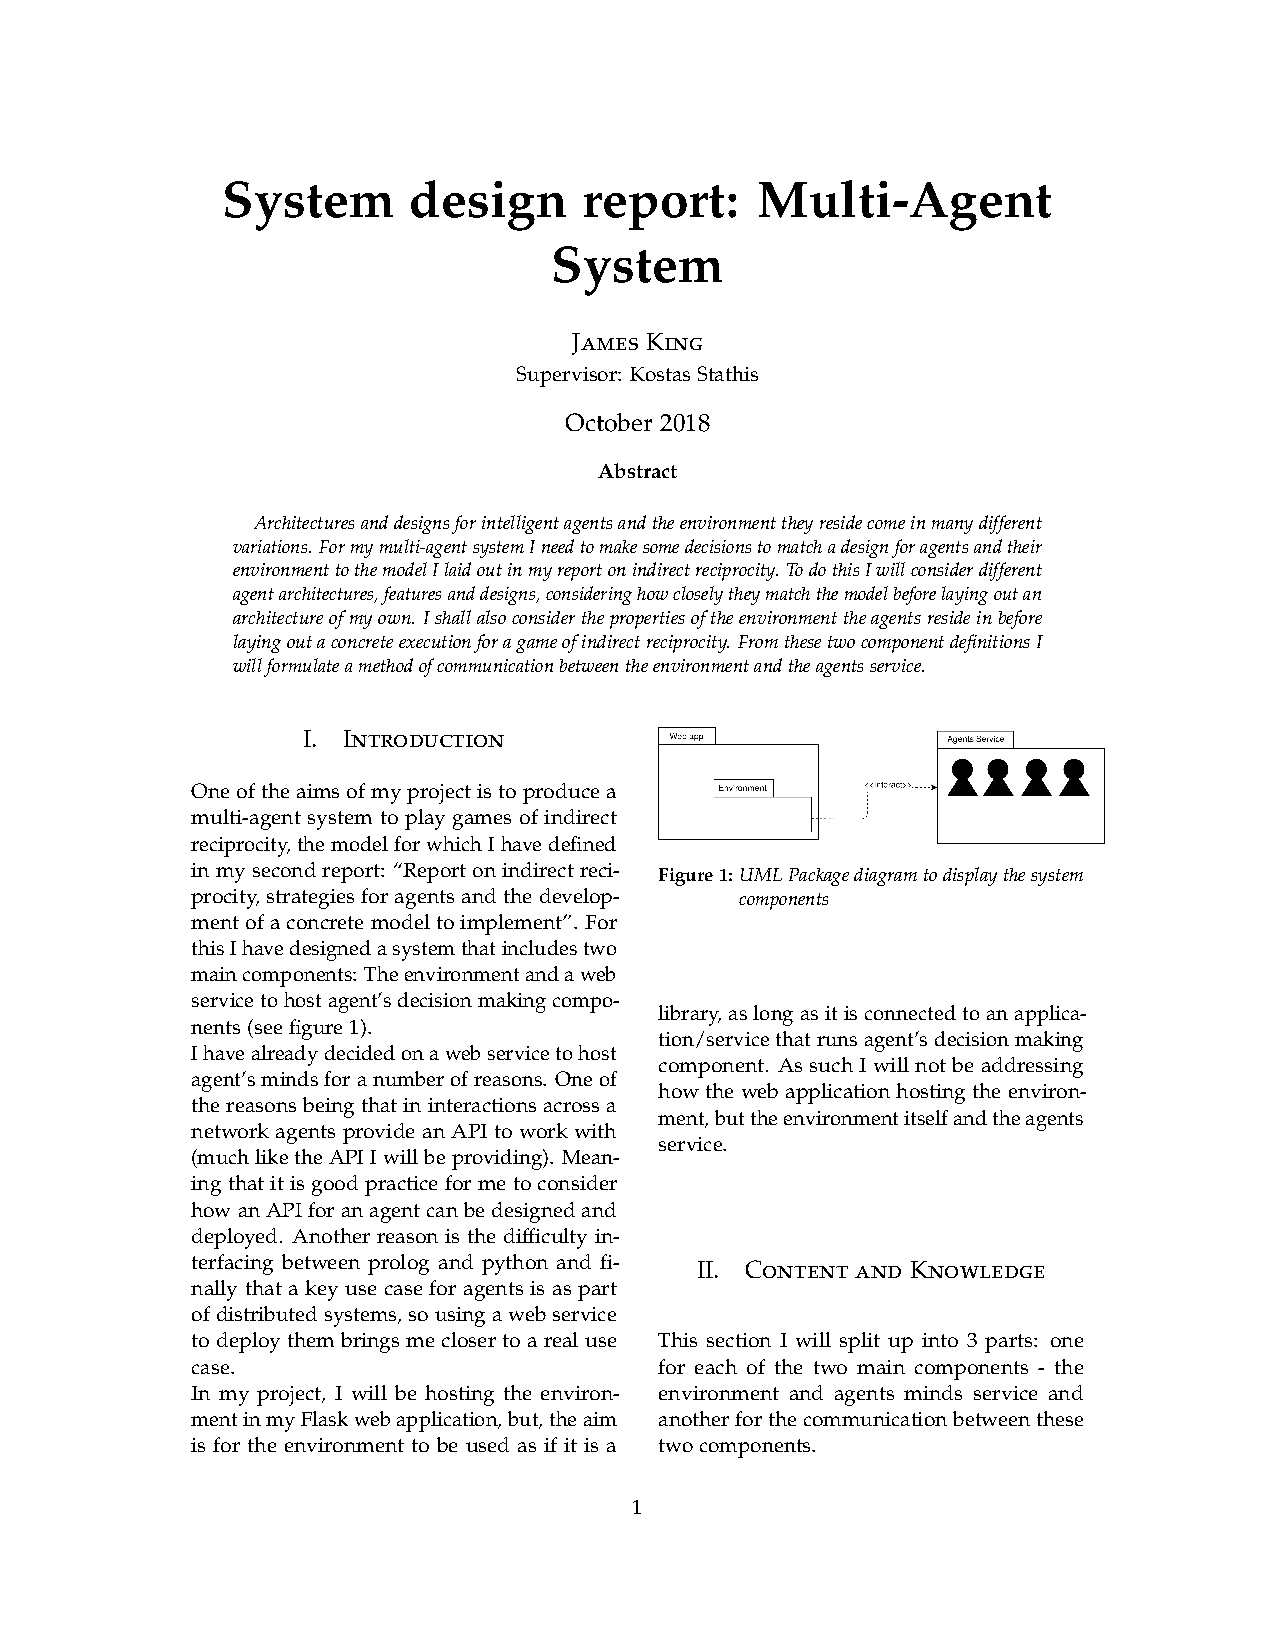
\includepdf[pages=-]{../../SysDesign/SysDesign.pdf}

%\begin{figure}
%	
\includepdf[pages=-,link=true,linkname=web_app_testing]{../../TestingStrategy/TestingStrategy.pdf}
%	\caption{\label{appendix:web_app_testing}}
	
%\end{figure}


\end{document}

\end{article}
